\documentclass{beamer}

\usepackage[utf8]{inputenc}
\usepackage{graphicx}
\usepackage{default}

\begin{document}
  \begin{frame}
    \frametitle{Introduction}
    Notre problème est de connaître le meilleur moyen pour chauffer rapidement une piscine. Pour cela, nous allons calculer les apports et pertes thermiques dans plusieurs cas, avant de les comparer. Nous étudierons tout d’abord le cas de la piscine seule. Ensuite, nous nous intéresserons aux cas où l’on couvre la piscine avec une bâche, puis deux bâches.
    %Content goes here
  \end{frame}
  \begin{frame}
   \frametitle{Hypothèses}
   	Afin de résoudre ce problème, nous avons dû faire un certain nombre d’hypothèses. 

Tout d’abord, nous ferons l’hypothèse que les parois de la piscine sont parfaitement isolées, ce qui implique que les seuls échanges de chaleur ont lieu à la surface de la piscine. De plus, le fond de la piscine est supposé assez foncé pour que l’intégralité du rayonnement solaire soit absorbé par la piscine ( et par la bâche lorsqu’il y en a une ).

Nous supposons aussi que les pertes thermiques par rayonnement de la piscine sont négligeables.

Nous considèrerons également, après avoir calculé la résistance thermique de la bâche, qu’il s’agit d’un solide ayant cette résistance thermique. 

Aussi, nous supposerons que la surface de l’eau est un solide, d’épaisseur infinitésimale.
  \end{frame}
  \begin{frame}
   \frametitle{schema}
   \begin{figure}[ht!]
    \centering
    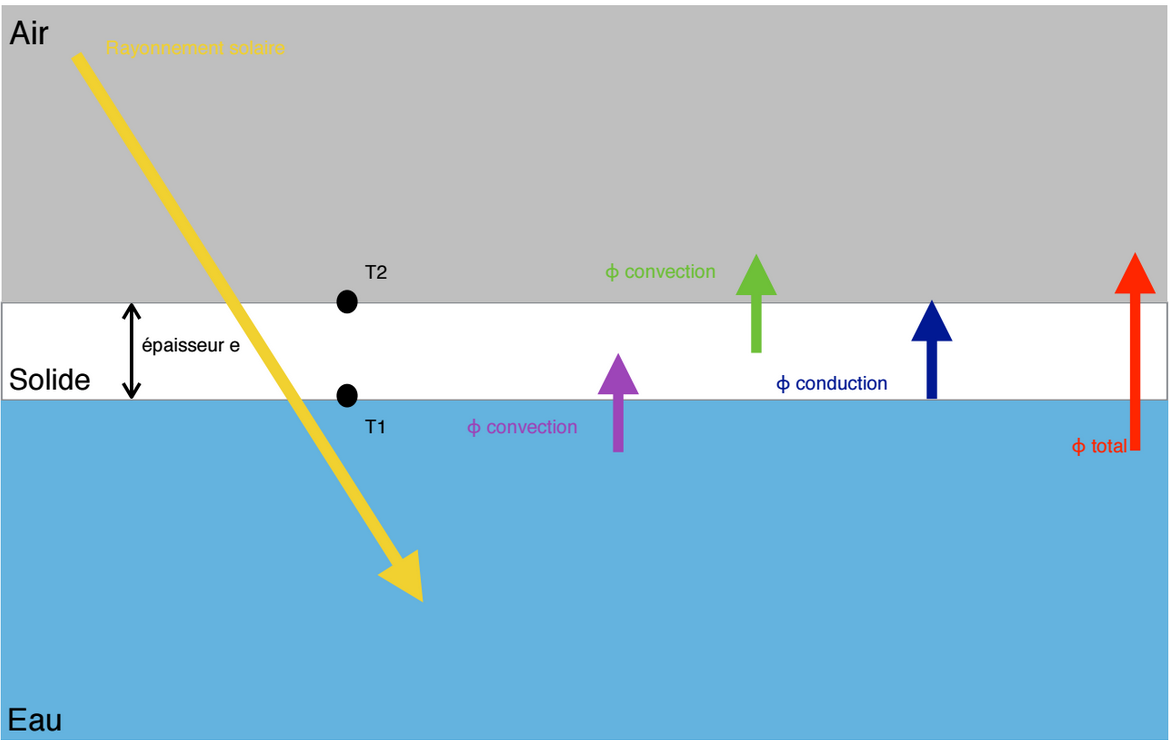
\includegraphics[width=90mm]{thermo.png}
    \caption{Mod\'{e}lisation du cas g\'{e}n\'{e}ral \label{overflow}}
   \end{figure}
  \end{frame}

  \begin{frame}
    \frametitle{This is the second slide}
    \framesubtitle{A bit more information about this}
    \[h_{eau}*S*(T_{eau} - T_{1}) = \phi_{convection(e->s}\]
    \[\frac{1}{R_{s}} * (T_{1} - T_{2}) = \phi_{conduction}\]
    \[h_{air}*S*(T_{2} - T_{air}) = \phi_{convection(s->air)}\]
    %More content goes here
  \end{frame}
  \begin{frame}
    \frametitle{This is the first slide}
    \[T_{eau} - T_{air} = T_{eau} - T_{1} + T_{1} - T_{2} - T_{air}\]
    \[T_{eau} - T_{air} = \frac{\phi_{convection(e->s)}}{h_{eau}*S} + \frac{\phi_{conduction}}{\frac{1}{R_{s}}} + \frac{\phi_{convection(s->air)}}{h_{air}*S} \]
    \[T_{eau} - T_{air} = \phi_{tot} * \frac{h_{air} + h_{eau}*h_{air}*S*R_{s} + h_{eau}}{h_{eau}*h_{air}*S}\]
    %Content goes here
  \end{frame}
  \begin{frame}
   \frametitle{Choix du codage en Python}
   Le flux dépend de la température et la température dépend du flux, comment faire ?
Nous avons écris un programme en python qui répète:
    \begin{enumerate}
     \item Calculer le flux à partir de la température
     \item Faire varier la température en soumettant l’eau au flux pendant une seconde

    \end{enumerate}

  \end{frame}

% etc
\end{document}
